\ifmostrarGabarito
\textbf{Resposta: (C)}

\textbf{Justificativa:}
Dicionários (\texttt{dict}) e conjuntos (\texttt{set}) em Python são implementados internamente por meio de **tabelas de dispersão (\emph{hash tables})**.
Isso permite que operações de pertinência e busca (\texttt{chave in dict} e \texttt{item in set}) ocorram em tempo médio constante $O(1)$, exigindo que as chaves/itens sejam objetos imutáveis (\emph{hashable}).
Em contrapartida, em listas (\texttt{list}), a busca \texttt{item in lista} exige percorrer elemento por elemento sequencialmente ($O(n)$).
\else
\par\vspace{0.15cm}
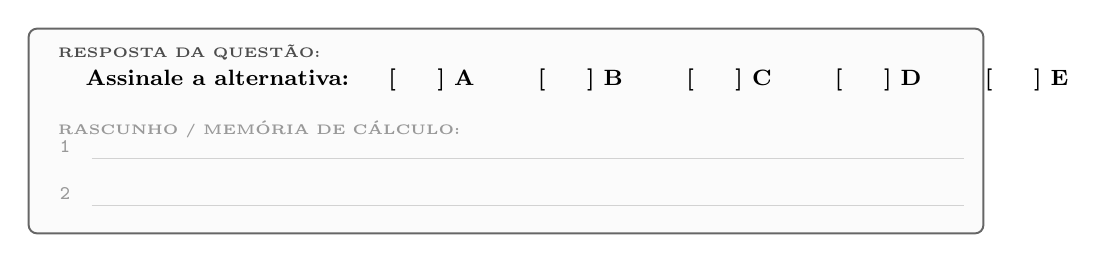
\begin{tikzpicture}
  \draw[rounded corners=3pt, draw=black!60, line width=0.7pt, fill=gray!3] (0,0) rectangle (\linewidth, -2.6cm);
  \node[anchor=north west, font=\tiny\bfseries\color{black!70}] at (0.25cm, -0.08cm) {RESPOSTA DA QUESTÃO:};
  \node[anchor=west, font=\footnotesize\bfseries] at (0.6cm, -0.65cm) {Assinale a alternativa: \quad [ \hspace{0.3cm} ] A \qquad [ \hspace{0.3cm} ] B \qquad [ \hspace{0.3cm} ] C \qquad [ \hspace{0.3cm} ] D \qquad [ \hspace{0.3cm} ] E};
  \node[anchor=north west, font=\tiny\bfseries\color{gray!80}] at (0.25cm, -1.05cm) {RASCUNHO / MEMÓRIA DE CÁLCULO:};
  \draw[gray!35, line width=0.4pt] (0.8cm, -1.65cm) -- (\linewidth-0.25cm, -1.65cm);
  \draw[gray!35, line width=0.4pt] (0.8cm, -2.25cm) -- (\linewidth-0.25cm, -2.25cm);
  \node[anchor=east, font=\scriptsize\ttfamily\color{gray!80}] at (0.65cm, -1.5cm) {1};
  \node[anchor=east, font=\scriptsize\ttfamily\color{gray!80}] at (0.65cm, -2.1cm) {2};
\end{tikzpicture}
\par\vspace{0.2cm}
\fi
